%%%%%%%%%%%%%%%%%%%%%%%%%%%%%%%%%%%%%%%%%%%%%%%%%%%%%%%%%%%%%%%%%%%%%%%%%
%%%%%%%%%%%%%%%%%%%%%%%%%%%%%%%%%%%%%%%%%%%%%%%%%%%%%%%%%%%%%%%%%%%%%%%%%
%%%%%%%%%%%%%%%%%%%%%%%%%%%%%%%%%%%%%%%%%%%%%%%%%%%%%%%%%%%%%%%%%%%%%%%%%
\section{Numerical Examples}\label{examples}

In this section we give some numerical examples to point out the properties of the piecewise rigid Finsler evolution. 

It should be noted that the resulting sequence $\{\Gamma_k\}$ depends on the choice of the step sizes $\{\tau_k\}$, which is left to the user and should only comply with the Wolfe conditions \eqref{Wolfe}.

Numerically, we observe in practice  that choosing small enough (according to the Wolfe condition) step sizes $\tau_k$ always provides consistent evolutions. This phenomenon is related to the existence of a limiting gradient flow (as highlighted in Remark \ref{grad_flow}), and the depicted evolutions are intended to show an approximation of this flow.



For the numerical examples shown in this section and in Section \ref{NE}, we used a fixed finite element discretization as detailed in Section \ref{discretization} (with $n=1280$). 
	This corresponds to 
 	imposing a fixed common parameterization of the discretized curves generated by the iterations. Note however that applications
	to more complicated imaging problems might require re-parameterizing the curves from time to time during the iterations
	of the gradient descent \eqref{sequence}. This is important when dealing with complicated shapes since the parameterization 
	might become ill-conditionned, 
	which can deteriorate the numerical accuracy of the scheme. 

%%%%%%%%%%%%%%%%%%%%%%%%%%%%%%%%%%%%%%%%%%%%%%%%%%%%%%%%%%%%%%%%%%%%%%%%%
\subsection{Influence of $\rho$} 
\label{sec-influ-rho}

To exemplify the main properties of the piecewise rigid Finsler flow, we introduce a synthetic example where we replace in the definition~\eqref{grad-rigid} of the Finsler gradient $\nabla_{R_\GA} E(\GA)$ (more precisely in the definition~\eqref{eq-dev-constr} of the constraint $\Ll_\Ga$) the  gradient $\nablad E(\Ga)$ by the vector field $F(\Ga) \in T_\Ga \Bb$ defined as
\eql{\label{field-const}
	F(\Ga) : s \in \Circ \mapsto -\pa{ 5\GA_1(s), 1000(\Ga_2(s)-1/2)^2} \in \RR^2
}
\eq{
	\qwhereq
	\Ga(s) = (\Ga_1(s),\Ga_2(s)) \in \RR^2.
}
The initial flow associated to this vector field reads
\eql{\label{eq-synthetic-flow}
	\Ga_{k+1} = \Ga_k - \tau_k F( \Ga_k )
}
for some small enough time steps $\tau_k>0$. Such a flow is represented in Figure~\ref{-F} where $\tau_k = 0.0005$ for every $k$.

\begin{figure}[!h]
\begin{center}
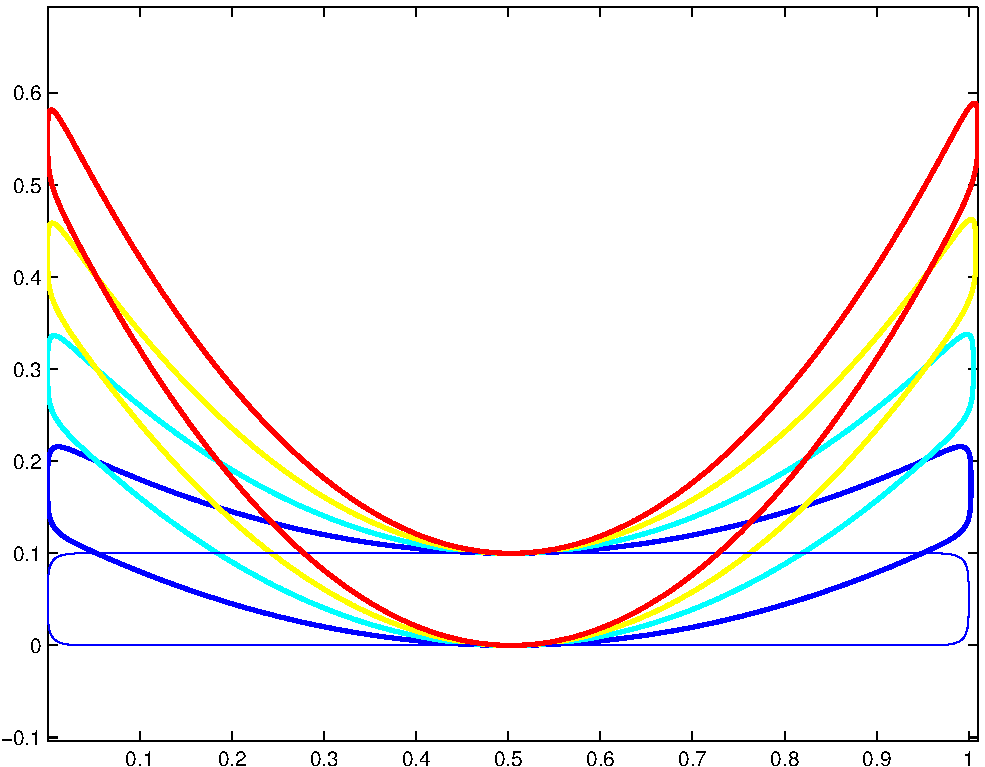
\includegraphics[width=.3\linewidth]{Field}
\end{center}
\caption{\label{-F} Evolution generated by $-F$. }
\end{figure}

Figure~\ref{fig1} shows the impact of the parameter $\rho$ on this evolution. As $\rho$ increases, the evolution becomes increasingly piecewise rigid. For $\rho$ large enough, it is globally rigid, i.e. satisfies~\eqref{eq-rigid-flow} and  $\nabla_{R_{\Ga_k}} E(\Ga_k) \in \Rr_{\Ga_k}$ for all $k$, where $\Rr_{\Ga}$ is defined in~\eqref{eq-rigid-vector-space}. 

\begin{figure}[!h]
\begin{center}
\begin{tabular}{@{}c@{\hspace{5mm}}c@{}}
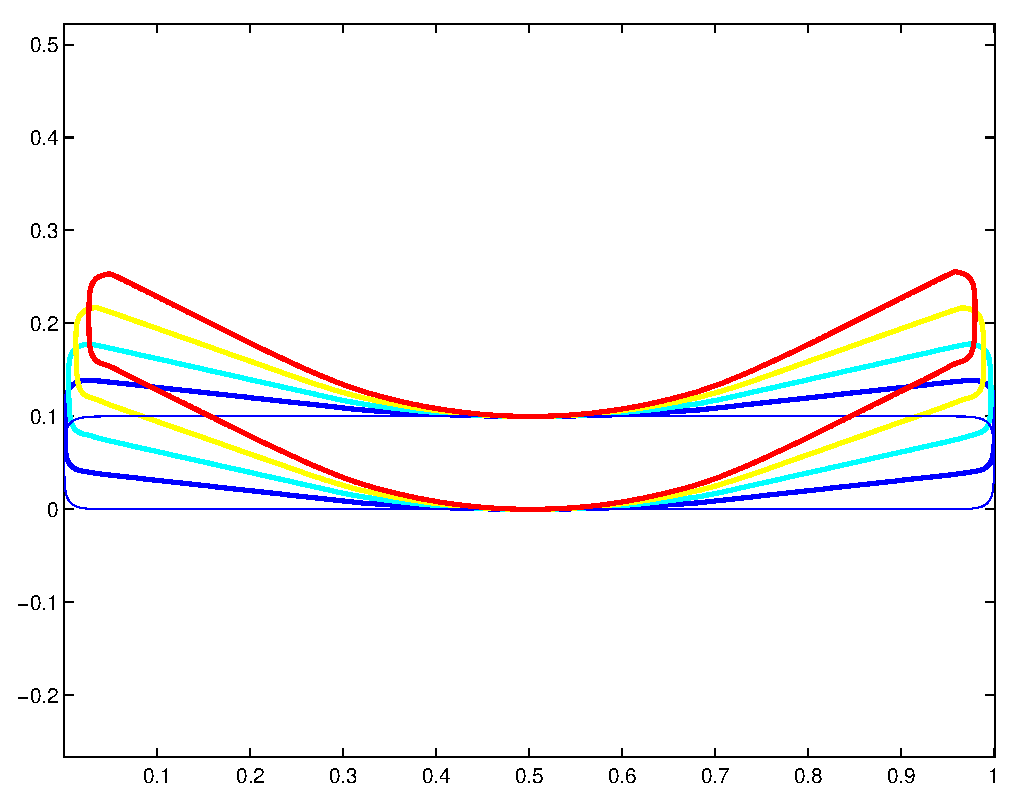
\includegraphics[width=.3\linewidth]{rod1-rho}&
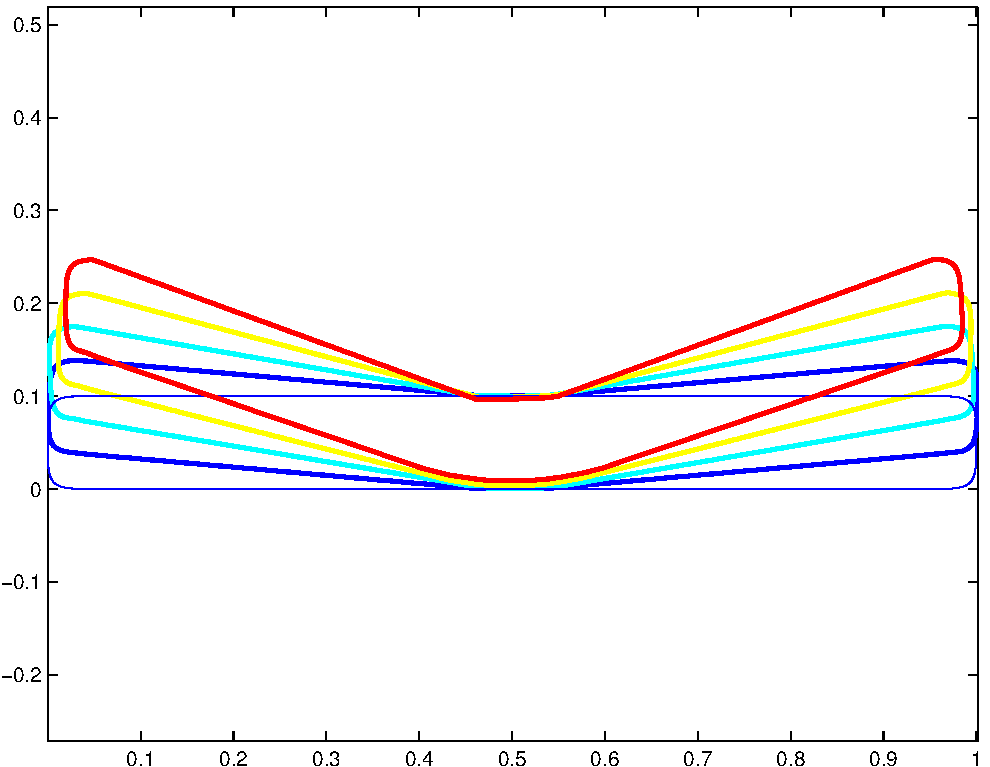
\includegraphics[width=.3\linewidth]{rod2-rho}\\
$\rho=0.1$ & $\rho= 0.3$ \\
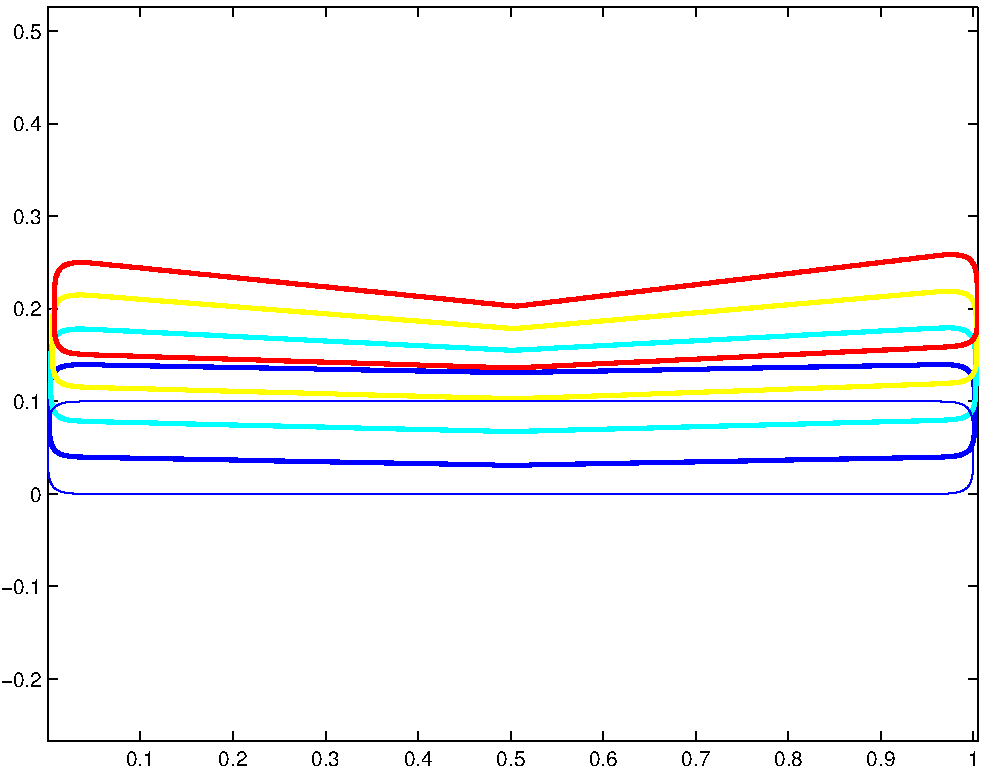
\includegraphics[width=.3\linewidth]{rod3-rho}&
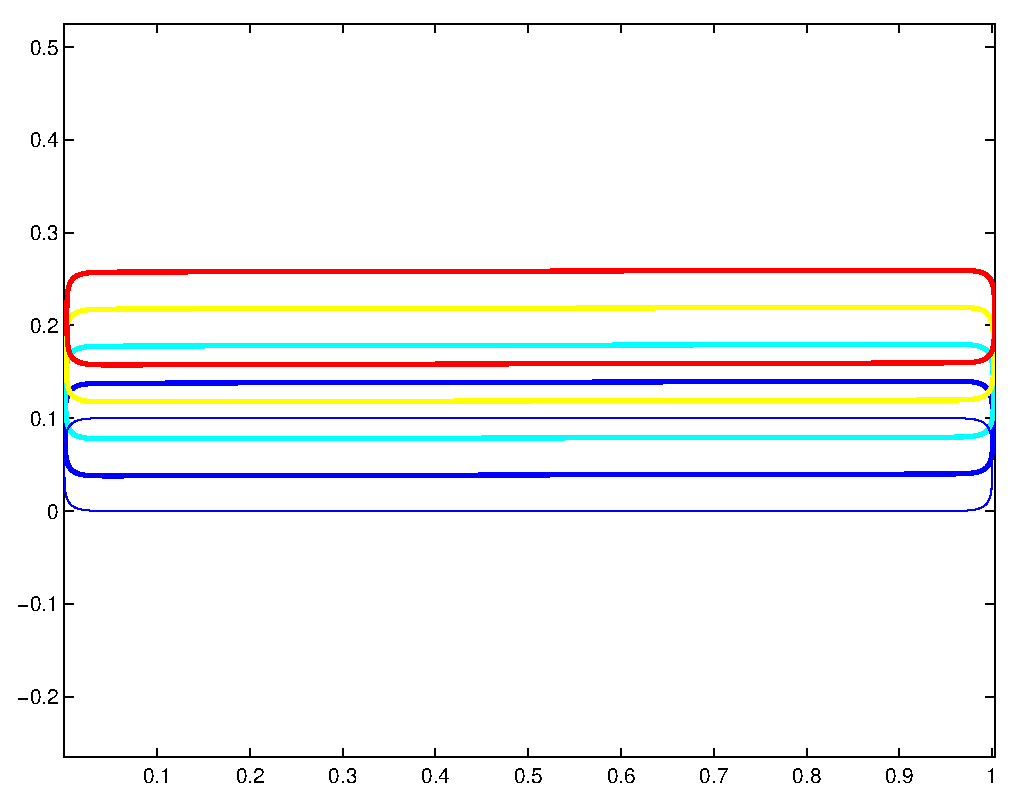
\includegraphics[width=.3\linewidth]{rod4-rho} \\
  $\rho= 0.7$  & $\rho=0.9$
\end{tabular}
\end{center}
\caption{\label{fig1} Evolution for different values of $\rho$. }
\end{figure}

%%%%%%%%%%%%%%%%%%%%%%%%%%%%%%%%%%%%%%%%%%%%%%%%%%%%%%%%%%%%%%%%%%%%%%%%%
\subsection{Curve Registration} 
\label{sec-numerics-registration}

We now give an example of application of the Finsler flow to the curve matching problem described in Section~\ref{CM}. Figure~\ref{evolutions0} compares the results of the piecewise-rigid Finsler gradient with the Sobolev Riemannian gradient detailed in Remark~\eqref{rem-fins-sob} which is very similar to the one introduced in~\cite{sundaramoorthi-sobolev-active,charpiat-generalized-gradient}. 
  
 
In order to obtain good matching results, it is important to select the parameters $(\tau,\si,\de)$ (see~\eqref{kernel} and~\eqref{eq-synthetic-flow}) in accordance to the typical size of the features of the curves to be matched.  For each method, we have manually tuned the parameters $(\tau,\si,\de)$ in order to achieve the best matching results. Choosing a large value of $\si$ and a smaller value for $\delta$ is useful to capture shapes with features at different scales, which is the case in our examples. 
 
\begin{figure}[h]
\centering
\begin{tabular}{@{}c@{\hspace{1mm}}c@{\hspace{1mm}}c@{\hspace{1mm}}c@{\hspace{1mm}}c@{}}
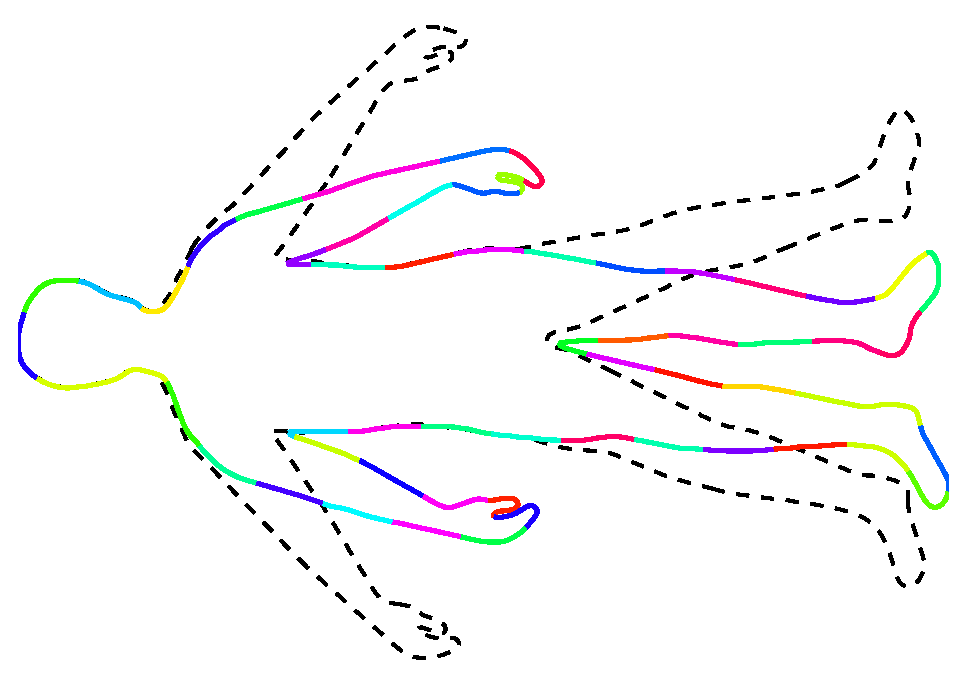
\includegraphics[height=.19\linewidth, angle=270]{man-finsler-rigid--initial}&
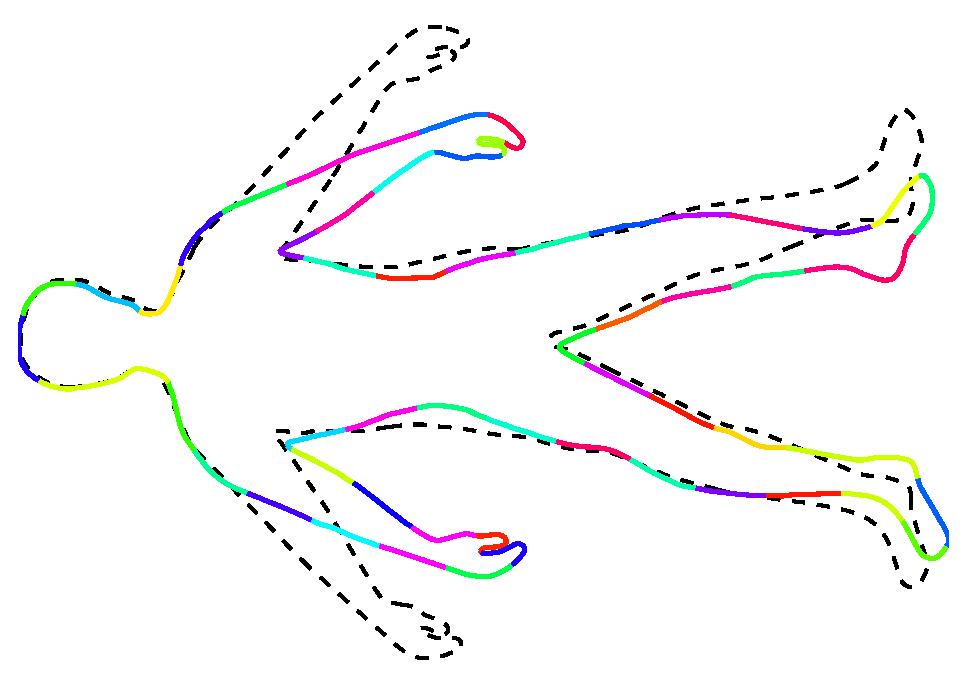
\includegraphics[height=.19\linewidth, angle=270]{man-finsler-rigid-5}&
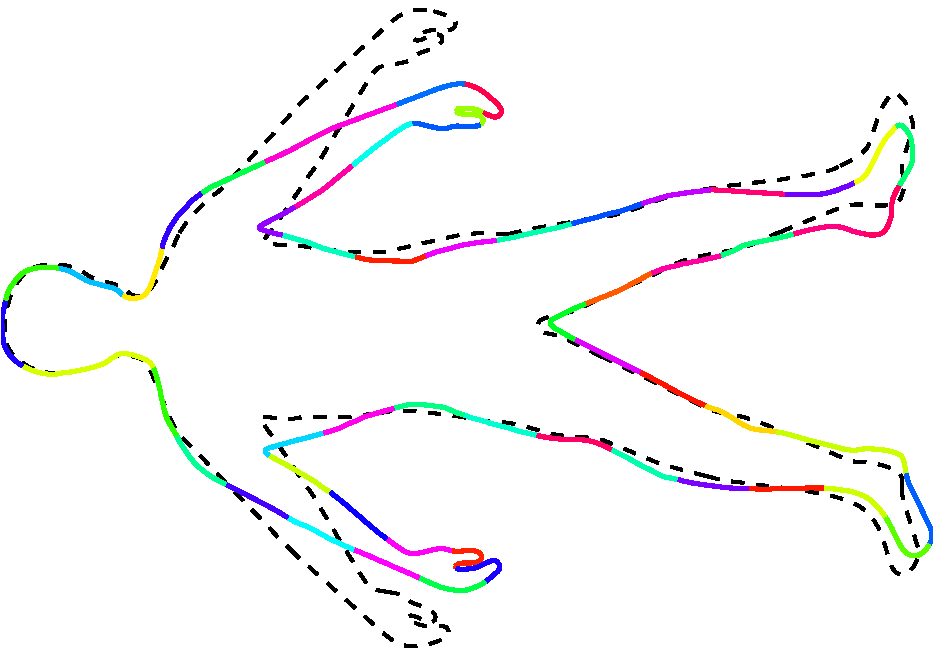
\includegraphics[height=.19\linewidth, angle=270]{man-finsler-rigid-8}&
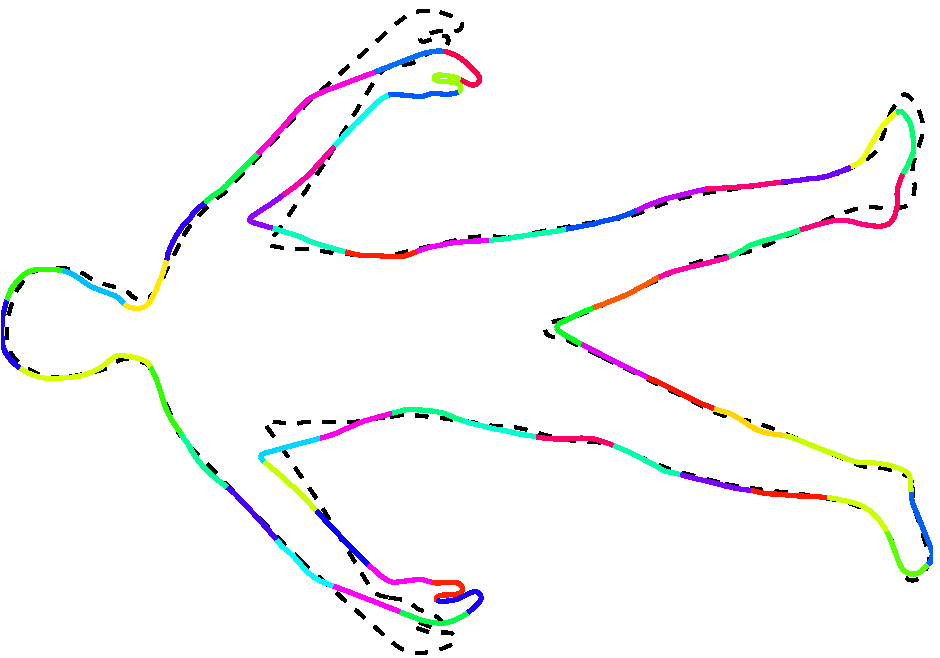
\includegraphics[height=.19\linewidth, angle=270]{man-finsler-rigid-18}&
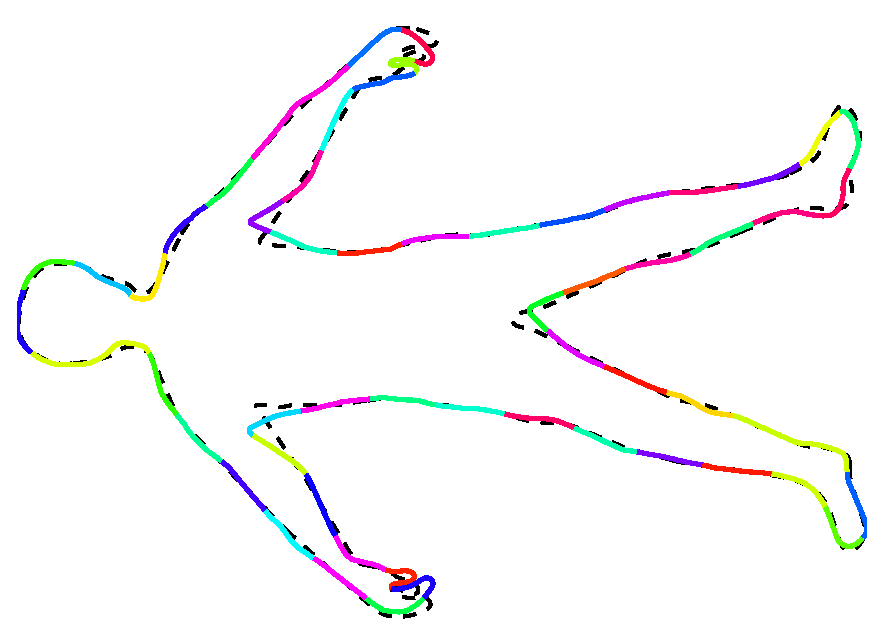
\includegraphics[height=.19\linewidth, angle=270]{man-finsler-rigid--final}\\
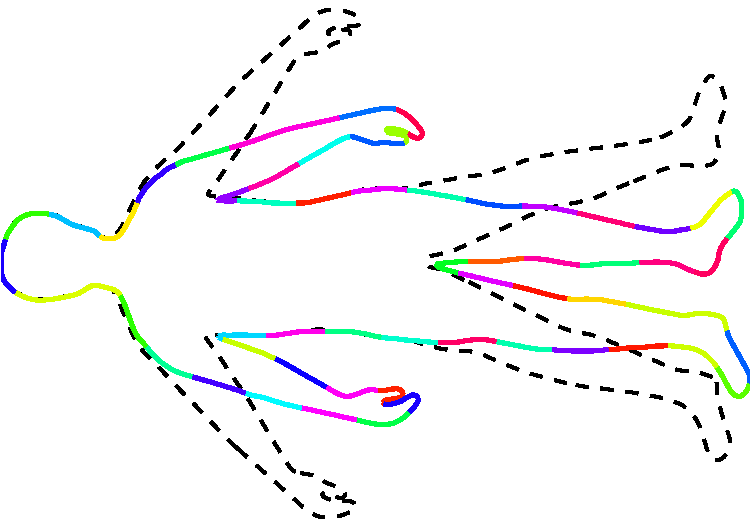
\includegraphics[height=.19\linewidth, angle=270]{man-bissobolev-initial}&
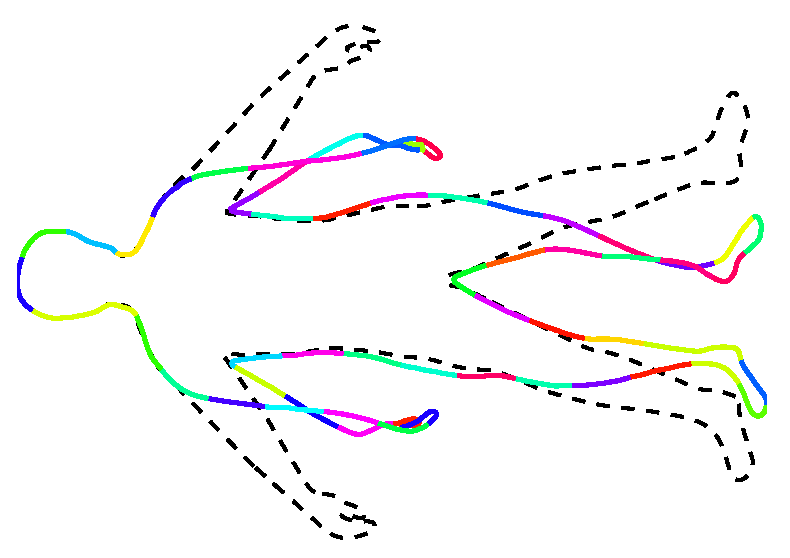
\includegraphics[height=.19\linewidth, angle=270]{man-bissobolev5}&
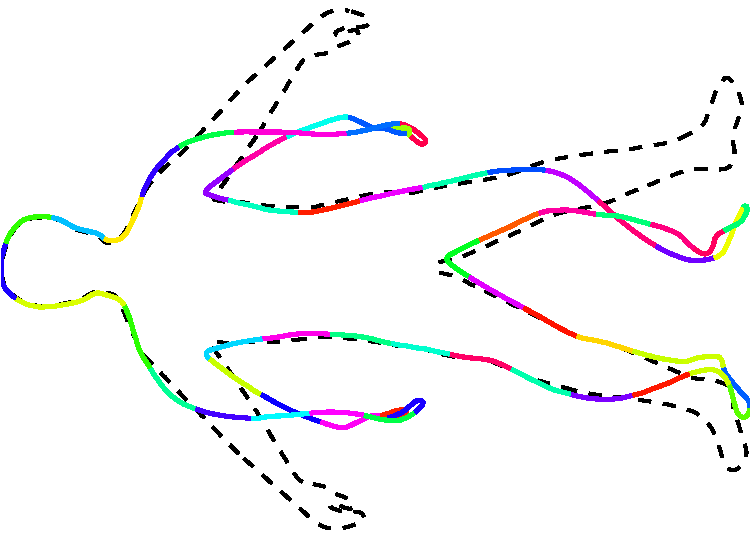
\includegraphics[height=.19\linewidth, angle=270]{man-bissobolev8}&
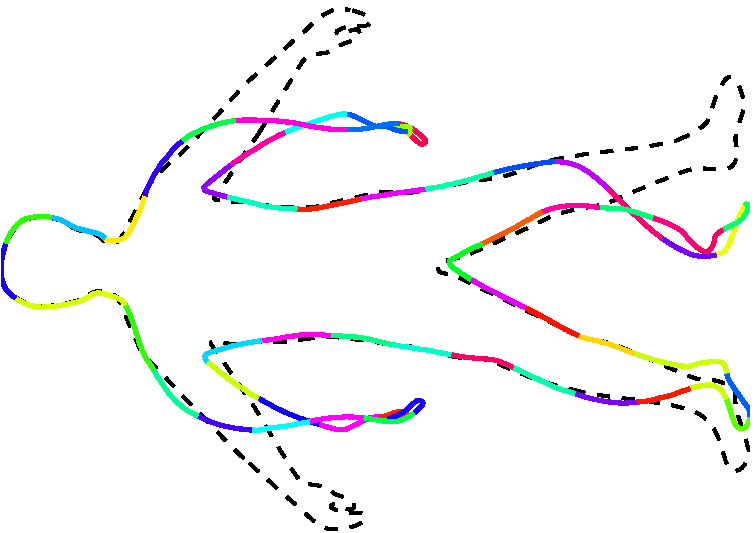
\includegraphics[height=.19\linewidth, angle=270]{man-bissobolev10}&
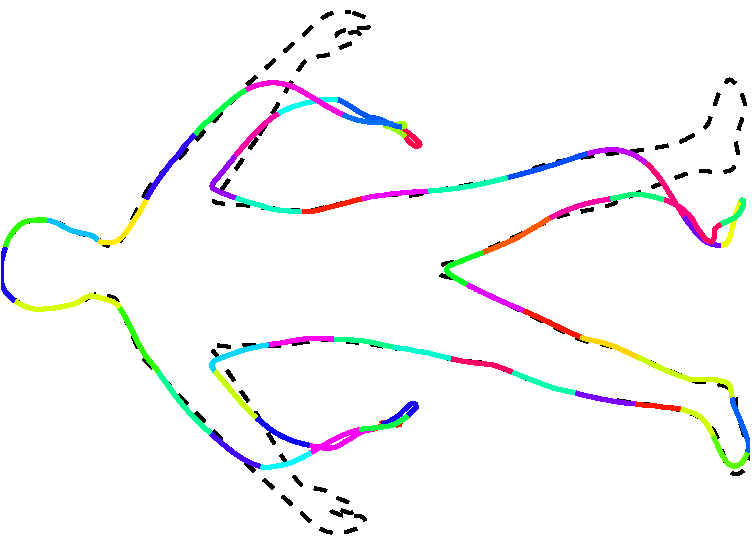
\includegraphics[height=.19\linewidth, angle=270]{man-bissobolev-final}
\end{tabular}
\caption{\label{evolutions0} Finsler evolution (top) with $\rho=0.8$ and  Sobolev evolution (bottom) for different step $k$ of the flow. Each image displays the target curve $\La$ (dash line) and the current curve $\Ga_k$ (solid line). The energy is computed using $\sigma=0.8$, $\delta=0.04$. }
\vspace{0.3cm}
\end{figure}

The piecewise rigid gradient is particularly efficient in this setting where the curves to be matched are naturally obtained by approximate articulations, which are well approximated by piecewise rigid deformations. Note however that our method does not necessitate a prior segmentation of the shape into disjoint areas undergoing rigid motions, i.e. the location of the articulations does not need to be known beforehand. The piecewise rigid matching is obtained solely by minimizing the distance energy $E(\Ga)$ to the target curve $\La$.  

The Finsler gradient thus allows to avoid poor local minima and perform an overall good global matching. In contrast the Sobolev gradient flow is trapped in a poor local minimum and the matching has failed. Note, however, that the matching achieved by the Finsler gradient is not perfect. Some local defects near corners are mostly due to the strong constraint $L_\Ga(\Phi)=0$ which enforces the exact conservation of the length of the curve. This constraint is alleviated in Section~\ref{similarity}, which presents a piecewise similarity Finsler gradient which leads to better matching results. 
